\documentclass[tikz]{standalone}
\usepackage{amsmath}
\definecolor{bg}{HTML}{171D2B}
\definecolor{aksen}{HTML}{F7B538}
\definecolor{teks}{HTML}{FFFFFF}
\definecolor{redcarry}{HTML}{F87171}
\definecolor{part}{HTML}{93C5FD}
\pagecolor{bg}
\begin{document}
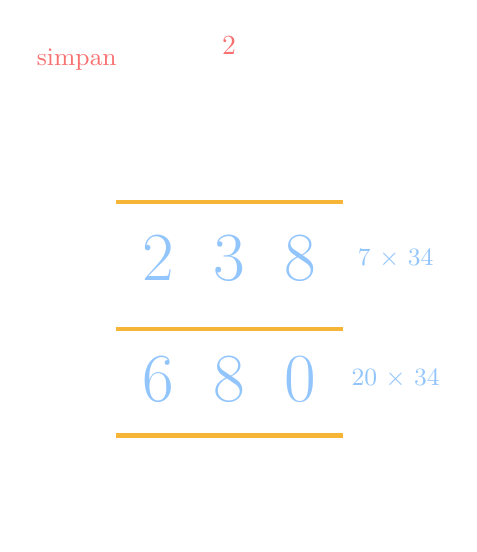
\begin{tikzpicture}[
  x=0.9cm, y=0.9cm,
  digit/.style={font=\Huge, text=teks},
  carry/.style={font=\normalsize, text=redcarry},
  partial/.style={font=\Huge, text=part},
  garis/.style={draw=aksen, line width=1.6pt}
]
% kolom: ratusan x=0, puluhan x=1, satuan x=2
% 34 x 27
\node[carry] at (-1.15,2.9) {\small simpan};
\node[carry] at (1,3.1) {2};   % simpan 2 dari 7x4=28
\node[digit] at (2,2.5) {4};
\node[digit] at (1,2.5) {3};
\node[digit] at (0.35,2.5) {\small $\times$};
\node[digit] at (2,1.5) {7};
\node[digit] at (1,1.5) {2};
% garis
\draw[garis] (-0.6,0.9) -- (2.6,0.9);
% baris parsial 1: 238 (7 x 34)
\node[partial] at (2,0.1) {8};
\node[partial] at (1,0.1) {3};
\node[partial] at (0,0.1) {2};
\node[font=\small, text=part] at (3.35,0.1) {7 $\times$ 34};
% garis
\draw[garis] (-0.6,-0.9) -- (2.6,-0.9);
% baris parsial 2: 680 (20 x 34, 0 di satuan)
\node[partial] at (2,-1.6) {0};
\node[partial] at (1,-1.6) {8};
\node[partial] at (0,-1.6) {6};
\node[font=\small, text=part] at (3.35,-1.6) {20 $\times$ 34};
% simpan 2 dari 8+8=16 puluhan? (tidak perlu; langsung jumlah)
% garis hasil
\draw[garis] (-0.6,-2.4) -- (2.6,-2.4);
\node[digit] at (2,-3.2) {8};
\node[digit] at (1,-3.2) {1};
\node[digit] at (0,-3.2) {9};
\node[digit] at (-1,-3.2) {1};
\node[font=\small, text=teks] at (3.35,-3.2) {hasil};
\end{tikzpicture}
\end{document}
